% !TeX spellcheck = en_US

% some nice styling for code listings
\definecolor{mygreen}{rgb}{0,0.6,0}
\definecolor{mygray}{rgb}{0.5,0.5,0.5}
\definecolor{mymauve}{rgb}{0.58,0,0.82}
\definecolor{lightgray}{rgb}{0.97,0.97,0.97}

\lstset{ %
	backgroundcolor=\color{lightgray},   % choose the background color; you must add \usepackage{color} or \usepackage{xcolor}
	basicstyle=\footnotesize,        % the size of the fonts that are used for the code
	breakatwhitespace=false,         % sets if automatic breaks should only happen at whitespace
	breaklines=true,                 % sets automatic line breaking
	captionpos=b,                    % sets the caption-position to bottom
	commentstyle=\color{mygreen},    % comment style
	deletekeywords={...},            % if you want to delete keywords from the given language
	escapeinside={\%*}{*)},          % if you want to add LaTeX within your code
	extendedchars=true,              % lets you use non-ASCII characters; for 8-bits encodings only, does not work with UTF-8
	frame=no,	                   % adds a frame around the code
	keepspaces=true,                 % keeps spaces in text, useful for keeping indentation of code (possibly needs columns=flexible)
	%keywordstyle=\color{blue},       % keyword style
	keywordstyle={},
	language=Octave,                 % the language of the code
	otherkeywords={*,...},           % if you want to add more keywords to the set
	numbers=left,                    % where to put the line-numbers; possible values are (none, left, right)
	numbersep=5pt,                   % how far the line-numbers are from the code
	numberstyle=\tiny\color{mygray}, % the style that is used for the line-numbers
	rulecolor=\color{black},         % if not set, the frame-color may be changed on line-breaks within not-black text (e.g. comments (green here))
	showspaces=false,                % show spaces everywhere adding particular underscores; it overrides 'showstringspaces'
	showstringspaces=false,          % underline spaces within strings only
	showtabs=false,                  % show tabs within strings adding particular underscores
	stepnumber=2,                    % the step between two line-numbers. If it's 1, each line will be numbered
	stringstyle=\color{mymauve},     % string literal style
	tabsize=2,	                   % sets default tabsize to 2 spaces
	title=\lstname                   % show the filename of files included with \lstinputlisting; also try caption instead of title
}

% helper for importing csv files with underscores
\newcommand{\expScore}{%
	\expandafter\expandafter\expandafter
	\detokenize
	\expandafter\expandafter\expandafter
}

\chapter{Simple demo \sbml models}
\section{Simple demo SBML version1}
\label{sec:appendix:simple-demo:v1}
\lstinputlisting[language=XML]{../supplementary/demo-sbml-simple/version1.xml}
\pagebreak

\section{Simple demo SBML version2}
\label{sec:appendix:simple-demo:v2}
\lstinputlisting[language=XML]{../supplementary/demo-sbml-simple/version2.xml}
\pagebreak

\section[Render of a Delta]{Complete render of the delta graph network}
\begin{figure}[H]
	\centering
	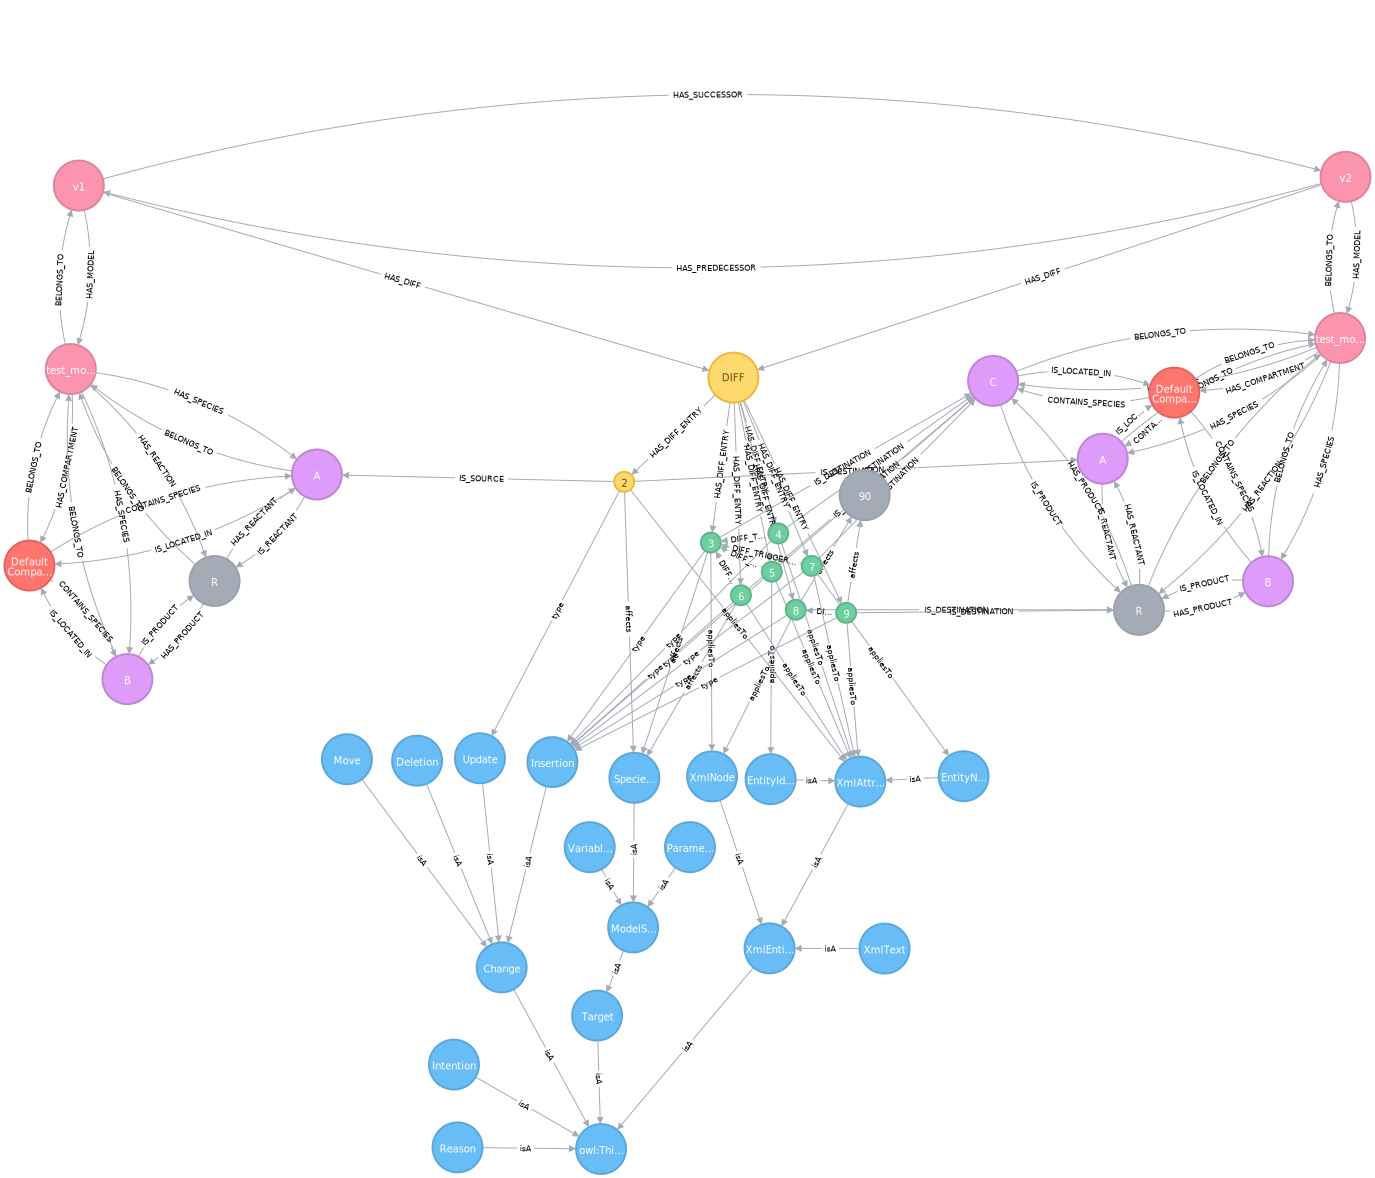
\includegraphics[width=\textwidth]{resources/neo4j-renders/demo-sbml-simple-diff-complete.pdf}
	\caption[\neoj graph representation of a delta between two demo models]{\neoj graph representation of a delta between two demo models. This is the full version of the simplified delta shown in Figure \ref{fig:results:simple-diff}}
	\label{fig:appendix:demo-sbml-simple-diff}
\end{figure}

\chapter{Representation of \comodi in \masymos}
\begin{figure}[H]
	\centering
	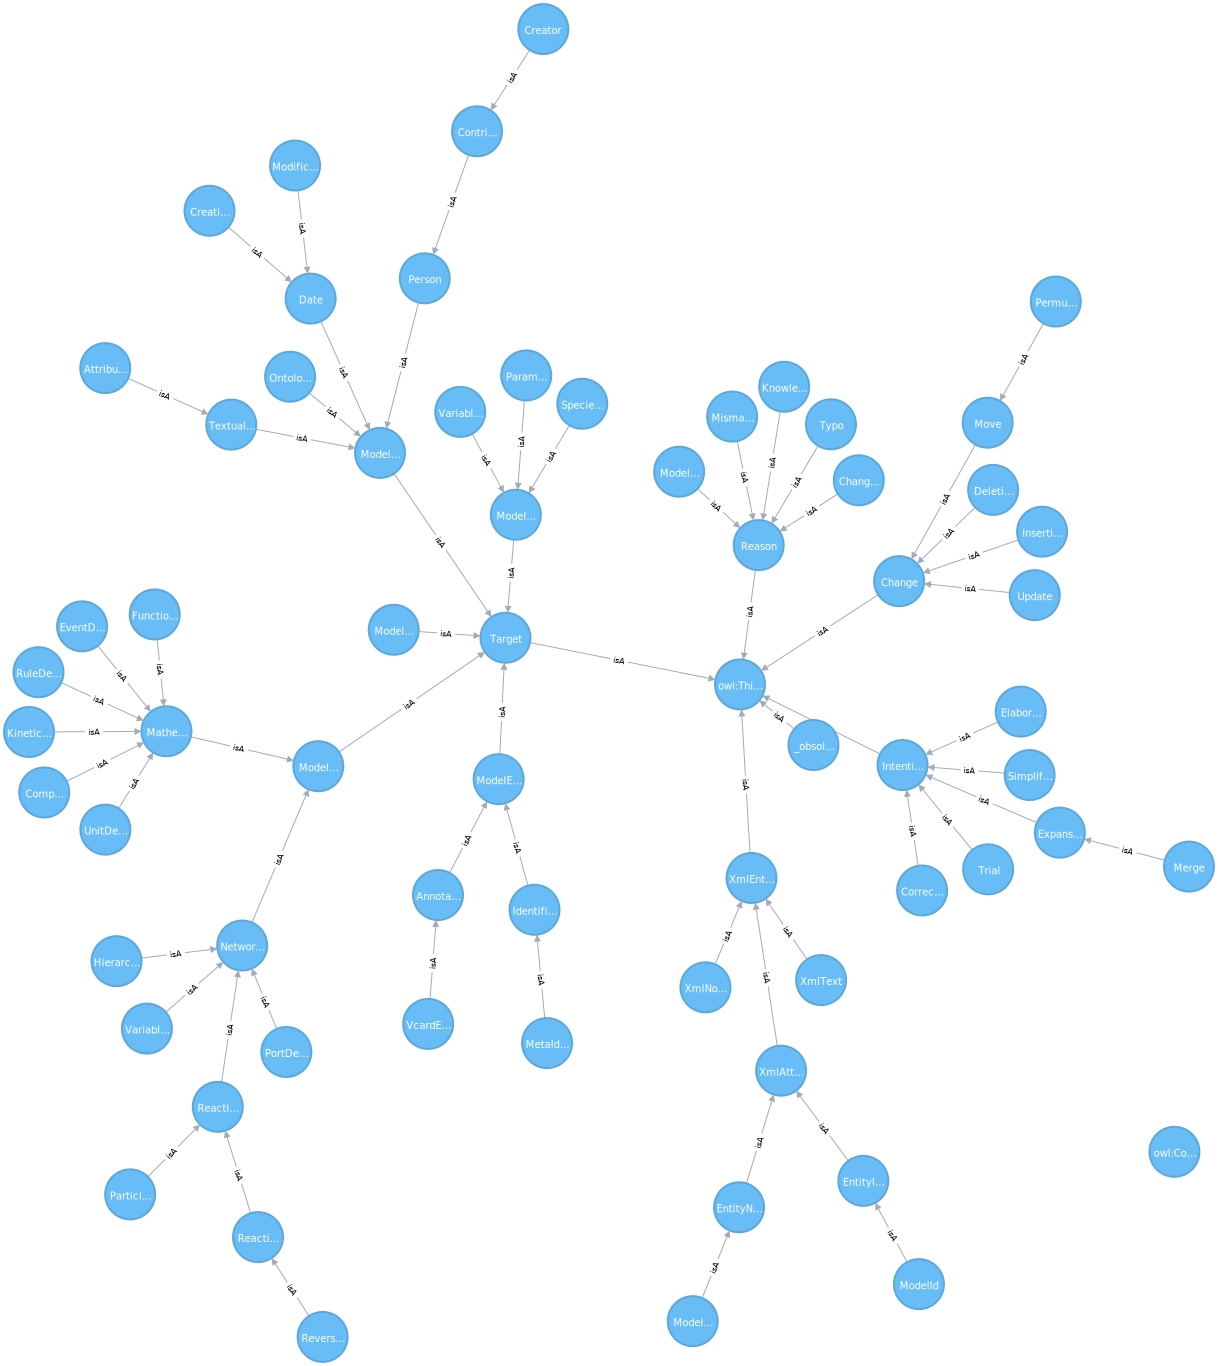
\includegraphics[width=\textwidth,height=0.5\textheight,keepaspectratio]{resources/neo4j-renders/comodi.pdf}
	\caption[Representation of \comodi in \masymos/\neoj]{Representation of \comodi in \masymos/\neoj. For the exact network refer to the documentation Figure \ref{fig:background:onto:comodi}}
	\label{fig:appendix:neo4j-comodi}
	\todo{make text larger/more readable?}
\end{figure}

\chapter{Overview of Node- and Relationship types}
\chaptermark{Node- and Relationship types}
\label{sec:appendix:meta-map}
\todo{write introduction thingy, where these numbers are coming from}

\section{Graphical Overview}
\begin{figure}[H]
	\centering
	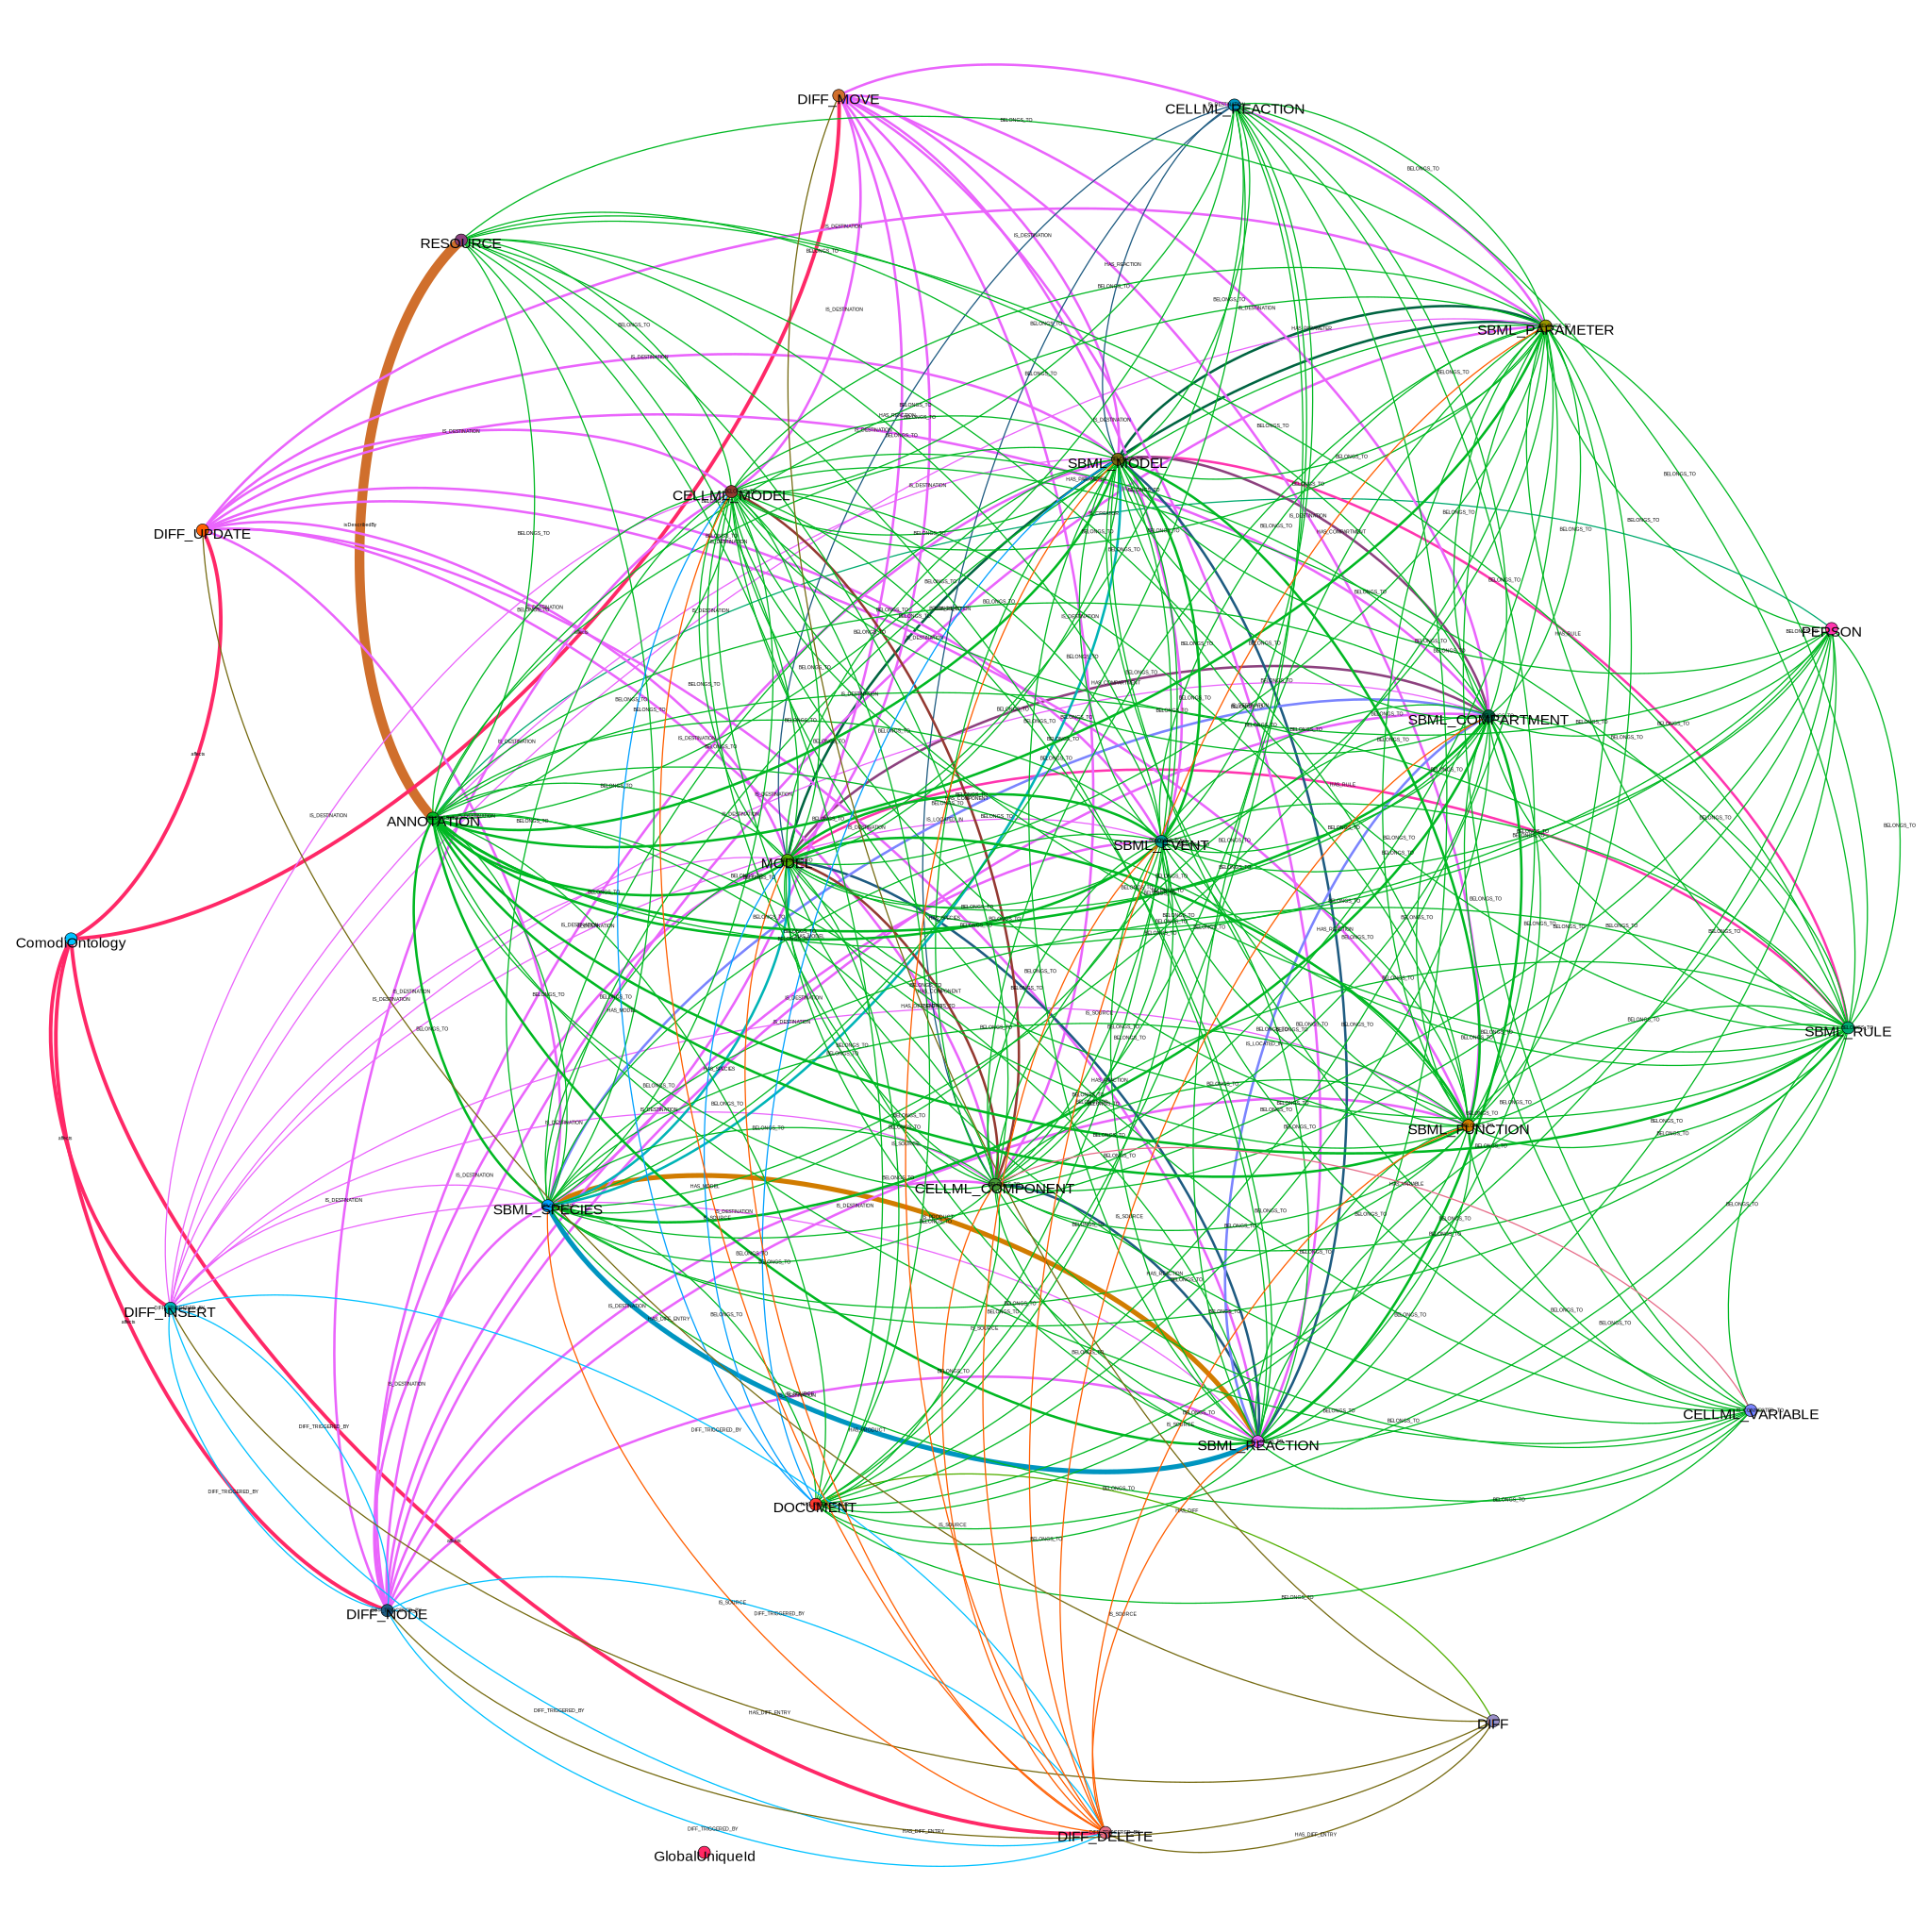
\includegraphics[width=\textwidth,height=0.5\textheight,keepaspectratio]{resources/neo4j-renders/large-test-meta-graph.pdf}
	\caption{Overview of all used node types and relations between them}
	\label{fig:appendix:meta-graph}
\end{figure}

\section{List of all used Node types}
\begin{longtable}{ l r }
	\hline \bfseries Node Label & \bfseries No. of occurrence \\\hline \endhead
	\csvreader[] %
	{resources/neo4j-renders/large-test-meta-graph-nodes.csv}{label=\nodeLabel,count=\count} %
	{\small \texttt{\expScore{\nodeLabel}} & \expScore{\count} \\} %
	%\hline
\end{longtable}

\section{List of all used Relationship types}
\begin{longtable}{ l c r }
	\hline \bfseries Source Node Label & \bfseries Relationship Type & \bfseries Destination Node Label \\\hline \endhead %
	\csvreader[]{resources/neo4j-renders/large-test-meta-graph-edges-expanded.csv}{Source=\sourceNode,Target=\targetNode,label=\relLabel} %
	{\texttt{\expScore{\sourceNode}} & \texttt{\expScore{\relLabel}} & \texttt{\expScore{\targetNode}} \\} %
	%\hline
\end{longtable}

\chapter{Compiling and Building the Prototype Implementation}
\chaptermark{Compiling and Building}

\section{Requirements and Dependencies}
Before attempting to compile and build the source, please make sure that following software packages are installed and working: \texttt{Git}, \texttt{JDK 1.8}, \texttt{Apache Maven 3}, \texttt{build-essentials}, \texttt{wget}, \texttt{curl}, \texttt{Python 3}, and \texttt{pip for Python 3}.

All described steps were developed and tested on \texttt{Linux 4.7.0-1-amd64 \#1 SMP Debian 4.7.8-1 (2016-10-19) x86\_64 GNU/Linux}. Alternative platforms might need adjustments to the build scripts or steps.

\section{Compiling and Building the Database}
% set some new settings for listings
\lstset{
	language=Bash,
	breaklines=true,
	breakatwhitespace=true,
	numbers=none,
	frame=single,
	framerule=0pt,
	belowskip=-24pt,
	aboveskip=5pt,
	basicstyle=\footnotesize\ttfamily,
	stringstyle={},
}

\begin{enumerate}
	\item Clone the repository from GitHub. This step can be skipped, if the material from the attached disc is used.
	\begin{enumerate}
		\item Open a terminal and navigate to a drive with at least 1GB of free disc space.
		\item Clone the main repository from GitHub:
\begin{lstlisting}
git clone git@github.com:FreakyBytes/bachelor-thesis.git
\end{lstlisting}
		\item Navigate into the newly cloned repository:
\begin{lstlisting}
cd bachelor-thesis
\end{lstlisting}
		\item Clone all git submodules:
\begin{lstlisting}
git submodule init
git submodule update
\end{lstlisting}
	\end{enumerate}

	\item Change into the \texttt{source} directory:
\begin{lstlisting}
cd source
\end{lstlisting}

	\item Start the build process:
\begin{lstlisting}
make all neo4j
\end{lstlisting}
		This command will invoke the build process for each subproject using Maven, also it will download, extract, and configure \neoj with all required dependencies. The resulting distribution can be found in the \texttt{neo4j} folder.
\end{enumerate}

\section{Populating the Database with Test Data}

\begin{enumerate}
	\item Open a terminal and navigate into the \texttt{source} directory, if not already done.
\begin{lstlisting}
cd source
\end{lstlisting}

	\item Make sure, that \neoj is not running:
\begin{lstlisting}
cd neo4j
bin/neo4j stop
cd ..
\end{lstlisting}

	\item Import the \comodi ontology using the \masymos-CLI:
\begin{lstlisting}
java -cp masymos-cli/target/masymos-cli-0.9.1.jar de.unirostock.sems.masymos.main.MainExtractor -dbPath ./neo4j/data/databases/graph.db -type owl -ontology ComodiOntology -directory ./COMODI/ontology/comodi.owl
\end{lstlisting}

	\item Start \neoj:
\begin{lstlisting}
cd neo4j
bin/neo4j start
\end{lstlisting}

	\item Change into the \texttt{ba-scripts} directory.
\begin{lstlisting}
cd ../../ba-scripts
\end{lstlisting}

	\item Install all \texttt{Python} dependencies, required for the \texttt{push2masymos} script:
\begin{lstlisting}
pip install -r requirements.txt
\end{lstlisting}

	\item Fill the database with test models, using the \texttt{push2masymos} script:
\begin{lstlisting}
python push2masymos.py --log=DEBUG -d test_models.yaml
\end{lstlisting}
	After all models are pushed the script will remain running and therefore continue to serve the model files via HTTP. This is important because the files need to be accessible in order to generate the diffs.

	\item Open a new terminal and trigger the diff generation using the \rest endpoint:
\begin{lstlisting}
curl -X POST http://localhost:7474/diff/service/trigger
\end{lstlisting}
	
	\item The progress can be observed using the \texttt{/stats} and \texttt{/status} endpoint:
\begin{lstlisting}
watch -n 10 "curl -X GET http://localhost:7474/diff/service/stats 2>/dev/null | python -m json.tool ; curl -X GET http://localhost:7474/diff/service/status 2>/dev/null | python -m json.tool"
\end{lstlisting}

	\item The \neoj web-interface is now available under:\\ \url{http://localhost:7474/browser/}
\end{enumerate}

